% =====================================================================
%  Research Design
%  ---------------------------------------------------------------------
%  This file is meant to be \input from your main document, e.g.:
%      \input{research-design}
%
%  Required packages (load these in your MAIN preamble):
%      \usepackage{amsmath}    % aligned equations, \text, \models, ...
%      \usepackage{graphicx}   % \includegraphics for the figures
%      \usepackage{booktabs}   % \toprule / \midrule / \bottomrule
%      \usepackage{tabularx}   % width-fitting validation table (pulls in array)
%
%  Notes:
%   * Figures use \includegraphics with the image files under images/.
%   * Cross-references WITHIN this file, to the literature review, and the
%     former <TBC> forward-reference are wired with \ref. References to
%     Appendix A, Appendix B and the Data and Results section are left as
%     plain text until those sections exist in the project.
%   * Table 1 (memory budget) has no data yet (placeholder table), and the
%     Keyword Generation candidate list is still "[to be added]".
% =====================================================================

\section{Research Design}
\label{sec:research-design}

\subsection{Design Approach}
\label{subsec:design-approach}

This section sets out the methodology for designing and evaluating the system in order to answer the project's stated research question. Accordingly, the research design was required to do two things: firstly, document a retrieval architecture in enough detail to be reproduced; secondly, define an evaluation methodology that establishes whether the architecture works and isolates the contribution of each component.

The following approach was used for systematically designing and validating the system:

\begin{enumerate}
    \item High-level design of the architecture, the graph schema, and the ingestion mechanism;
    \item Detailed design of each retrieval module;
    \item Isolated validation of each module against an appropriate benchmark;
    \item Validation of the integrated system against the research question.
\end{enumerate}

This ensures that each design decision made in the earlier stages has a corresponding benchmark in the later stages. The earlier stages document the design for reproducibility, and the later stages test it for validity. This correspondence is what makes the methodology suitable for this thesis.

Validating components in isolation also addresses a specific risk in this pipeline. Because each query passes through several components in sequence, an error observed at the output could originate in any one of them, and an end-to-end test alone cannot identify which. Validating each component separately removes that ambiguity, measuring the contribution of each rather than confounding them.

\subsection{System Architecture}
\label{subsec:system-architecture}

\begin{figure}[htbp]
    \centering
    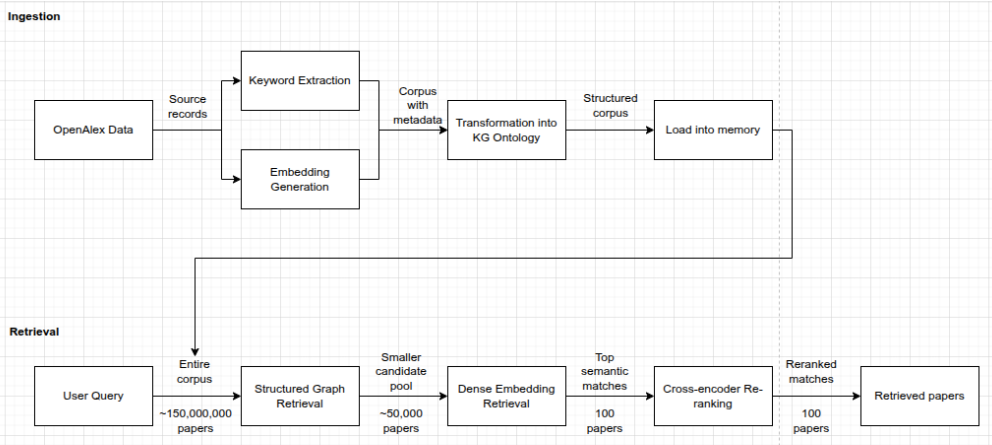
\includegraphics[width=\linewidth]{images/system_architecture.png}
    \caption{System architecture. An ingestion pipeline builds the knowledge graph that a three-stage retrieval cascade queries. The candidate pool size is illustrative and varies by query.}
    \label{fig:system-architecture}
\end{figure}

The system has two parts. An offline ingestion pipeline builds the knowledge graph from source data, and an online retrieval pipeline answers queries against it in three stages. Figure~\ref{fig:system-architecture} shows the overall design.

At a high level, the system uses an ingestion pipeline that:

\begin{itemize}
    \item takes OpenAlex as the source of paper data, namely the title, abstract, authors, and publication date of each work;
    \item extracts the keyphrases and dense embedding of each work from its title and abstract;
    \item transforms the data into the ontology chosen to represent the scholarly domain;
    \item loads the result into the database.
\end{itemize}

OpenAlex was chosen as the source because it is the largest fully open scholarly index and is the successor to the Microsoft Academic Graph, as established in Section~\ref{subsec:kg-infrastructure}. The keyphrases and embeddings extracted in this stage are not incidental products. They are the data that the first and second retrieval stages depend on. How each field is sourced and extracted, and the schema the data is transformed into, are documented in Section~\ref{subsec:component-design}.

For retrieval, the system uses a three-stage pipeline:

\begin{itemize}
    \item Structured graph retrieval, which produces the initial candidate pool. A natural-language query is translated into a structured representation of the keywords to search for and the Boolean logic that combines them, with keywords taken either from the query or from explicit user input. These keywords are matched against the graph's keyword nodes using BM25, and the papers attached to the matched nodes are retrieved and combined under the requested AND, OR, and NOT logic.
    \item Dense embedding retrieval, which narrows the candidate pool by semantic similarity. The query and each candidate paper are represented as high-dimensional vectors, and the candidates closest to the query by cosine similarity are kept, up to the top 100.
    \item Cross-encoder re-ranking, which orders the final results by relevance. A cross-encoder takes the query and a paper's title and abstract together and returns a single relevance score, and the top 100 from the second stage are re-ranked by that score.
\end{itemize}

This extends the two-stage retrieve-then-rerank pattern common to large-scale retrieval systems, placing a knowledge-graph candidate selector in front of the embedding-retrieval and cross-encoder re-ranking stages. Because the three stages increase in both accuracy and cost, each runs over a smaller set than the last, which is necessary because the most accurate stage cannot be run over the full corpus.

Each stage also performs a function the others cannot, which is why all three are present rather than any one alone. The first stage lets the system express typed or structural queries that the other two cannot. As established in Section~\ref{sec:lr-dense}, single-vector dense retrieval cannot represent requests such as papers from a particular author on a given topic published after a given year. Structured retrieval expresses these directly and returns a high-recall candidate set for the later stages to rank. Its output is unbounded. The structured representation and its compilation into a graph query are documented in Section~\ref{subsec:component-design}.

The second stage ranks that candidate set by semantic similarity, which structured retrieval cannot do, since it matches only on shared keywords. Dense embeddings rank candidates by their semantic relatedness to the full query, capturing relevance that exact-term matching misses. Section~\ref{sec:lr-dense} also showed that dense retrieval used alone misses a substantial share of relevant papers and is weak on entity-heavy queries, which is why it ranks a structured candidate set here rather than serving as the primary retrieval mechanism. The embeddings are quantised to reduce their memory footprint, with the quantisation and its justification documented in Section~\ref{subsec:component-design}.

The third stage refines the ranking once more. A bi-encoder compares two vectors that were computed separately, whereas a cross-encoder reads the query and the document together and can weigh their interaction directly, which Section~\ref{sec:lr-dense} identified as the source of the accuracy that late-interaction and cross-encoder approaches achieve over single-vector retrieval. This makes it more accurate but too expensive to run over many papers, which is why it is placed last and applied only to the 100 candidates the earlier stages have selected.

\subsection{Component Design}
\label{subsec:component-design}

\subsubsection{Knowledge Graph Schema}
\label{subsubsec:kg-schema}

\begin{figure}[htbp]
    \centering
    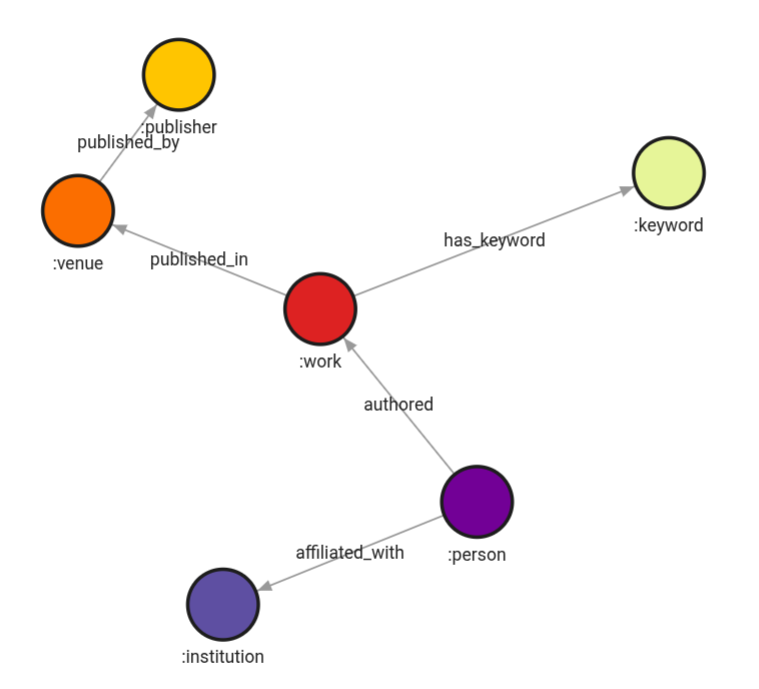
\includegraphics[width=\linewidth]{images/Schema.png}
    \caption{Scholarly Knowledge Graph Schema.}
    \label{fig:kg-schema}
\end{figure}

The schema is general purpose, built from generic entities such as works, keywords, and authors, so that it generalises beyond any single domain despite the biomedical focus of the data it is deployed on.

The design was derived from the knowledge graphs surveyed in Section~\ref{subsec:kg-infrastructure}, which commonly share a similar sub-ontology over the six node types required for retrieval (Work, Person, Institution, Venue, Publisher, and Keyword) and their associated edges. This schema is based on that common structure.

The main point of departure concerns keyword modelling. SemOpenAlex, which is also built on OpenAlex, attaches keywords to the topics assigned to works rather than to the works directly, because OpenAlex derives its keywords at the topic level. Since this schema derives its own keywords per work (Section~\ref{subsubsec:ingestion-storage}), it attaches them directly to the work rather than through a topic node. The resulting schema is shown in Figure~\ref{fig:kg-schema}.

The properties held on each node were refined through internal testing and reduced to the current set, which is given in Appendix~A.

\subsubsection{Ingestion and Storage}
\label{subsubsec:ingestion-storage}

For all purposes excluding benchmarks, the complete OpenAlex snapshot was used as the data source. As established in Section~\ref{subsec:kg-infrastructure}, OpenAlex is the most suitable index due to its large corpus of works and pre-processed metadata.

A biomedical subset was then selected from this snapshot by filtering on the OpenAlex field tag and retaining eleven fields, namely Medicine; Agricultural and Biological Sciences; Biochemistry, Genetics and Molecular Biology; Psychology; Health Profession; Chemistry; Neuroscience; Immunology and Microbiology; Nursing; Pharmacology, Toxicology and Pharmaceutics; and Dentistry. This subset gives the deployed system its biomedical focus, while the schema itself remains general purpose.

For each work in the subset, a keyword generation module and an embedding generation module produce the per-work keywords and the dense embedding that the structured and dense retrieval stages depend on. A number of models for each were benchmarked to inform the selection process, as outlined in Section~\ref{subsec:evaluation-validation}.

The resulting data was transformed to the structure of the ontology, and loaded into Memgraph using their documented best practices. Memgraph was used as an in-memory graph database, on a virtual machine provisioned with sufficient memory to hold the full graph. Memgraph was chosen for the query performance of an in-memory store at this scale, for its MAGE library of graph algorithms, and for a licence compatible with the intended use. Because the graph resides in memory, the dense embeddings are quantised from 32-bit floating point to 8-bit integers to fit within the available memory (see Table~\ref{tab:bienc-deploy} for the resulting footprint).

\subsubsection{Structured Graph Retrieval}
\label{subsubsec:structured-retrieval}

The first retrieval stage turns a natural-language query into a Memgraph-compatible Cypher query through a sequence of learned and deterministic sub-modules.

The query is first normalised, which collapses whitespace, resolves year hints into year bounds, and pulls out quoted phrases as exact-match terms, preserving case so that proper nouns and acronyms survive.

The normalised query is then converted into an Intermediate Representation (IR) using an LLM via a forced tool call whose schema mirrors the representation. The IR couples two components: firstly, a flat list of typed entities, each carrying a type, value, confidence and exact flag; secondly, a recursive boolean expression over those entities using AND, OR and NOT. This design aims to decouple LLM-based intent extraction from deterministic query construction, taking the flexibility of the former whilst keeping the correctness guarantee of the latter, as noted in Section~\ref{sec:lr-nl2q}. The representation is then validated, dropping low-confidence entities and rejecting any query with no entities to anchor the traversal.

The deterministic compiler turns the validated representation into Cypher. Rather than translating the boolean tree into nested graph patterns, it runs one subquery per entity, matching non-exact entities with BM25 over a text index and exact entities by direct property match. It then keeps each work whose matched entities satisfy the boolean expression.

Formally, for each entity $e_{i}$, let $W_{i}$ be the set of works that match it, subject to the work-level filters. Satisfaction of an expression $\varphi$ by a work $w$, written $w \models \varphi$, is defined by recursion over the structure of $\varphi$,
%
\begin{align*}
    w \models e_{i} &\quad\text{iff}\quad w \in W_{i}, \\
    w \models \mathrm{AND}(\varphi_{1}, \ldots, \varphi_{k}) &\quad\text{iff}\quad w \models \varphi_{j} \text{ for every } j, \\
    w \models \mathrm{OR}(\varphi_{1}, \ldots, \varphi_{k}) &\quad\text{iff}\quad w \models \varphi_{j} \text{ for some } j, \\
    w \models \mathrm{NOT}(\varphi) &\quad\text{iff}\quad \lnot\,(w \models \varphi).
\end{align*}
%
The leaves $e_{i}$ are the query's entities and $E$ is its full boolean expression, so the candidate set returned by the stage is
%
\[
    \{\, w \in \bigcup_{i} W_{i} \mid w \models E \,\},
\]
%
where $\bigcup_{i} W_{i}$ is the set of works matching at least one entity. Restricting the universe in this way ensures that a NOT excludes works within the matched set rather than admitting the works that match nothing, and the recursion preserves arbitrary nesting of the operators.

The compiled query runs against the database and returns the candidate pool together with its total match count. A worked example of a query, its intermediate representation, and the compiled Cypher is given in Appendix~B.
% Note: this is what they should look like when compiled.

\subsubsection{Dense Embedding Retrieval and Re-ranking}
\label{subsubsec:dense-rerank}

The second and third stages, dense embedding retrieval and cross-encoder re-ranking, are established techniques rather than novel contributions of this work, and their role within the cascade is described in Section~\ref{subsec:system-architecture}. The retrieve-then-rerank pattern they follow is reviewed in Section~\ref{sec:lr-dense}. The embedding and cross-encoder models are each selected by the benchmarking in Section~\ref{subsec:evaluation-validation}, and the generation and quantisation of the embeddings, together with the memory budget, are covered in Section~\ref{subsubsec:ingestion-storage}.

\subsection{Evaluation and Validation Design}
\label{subsec:evaluation-validation}

\begin{figure}[htbp]
    \centering
    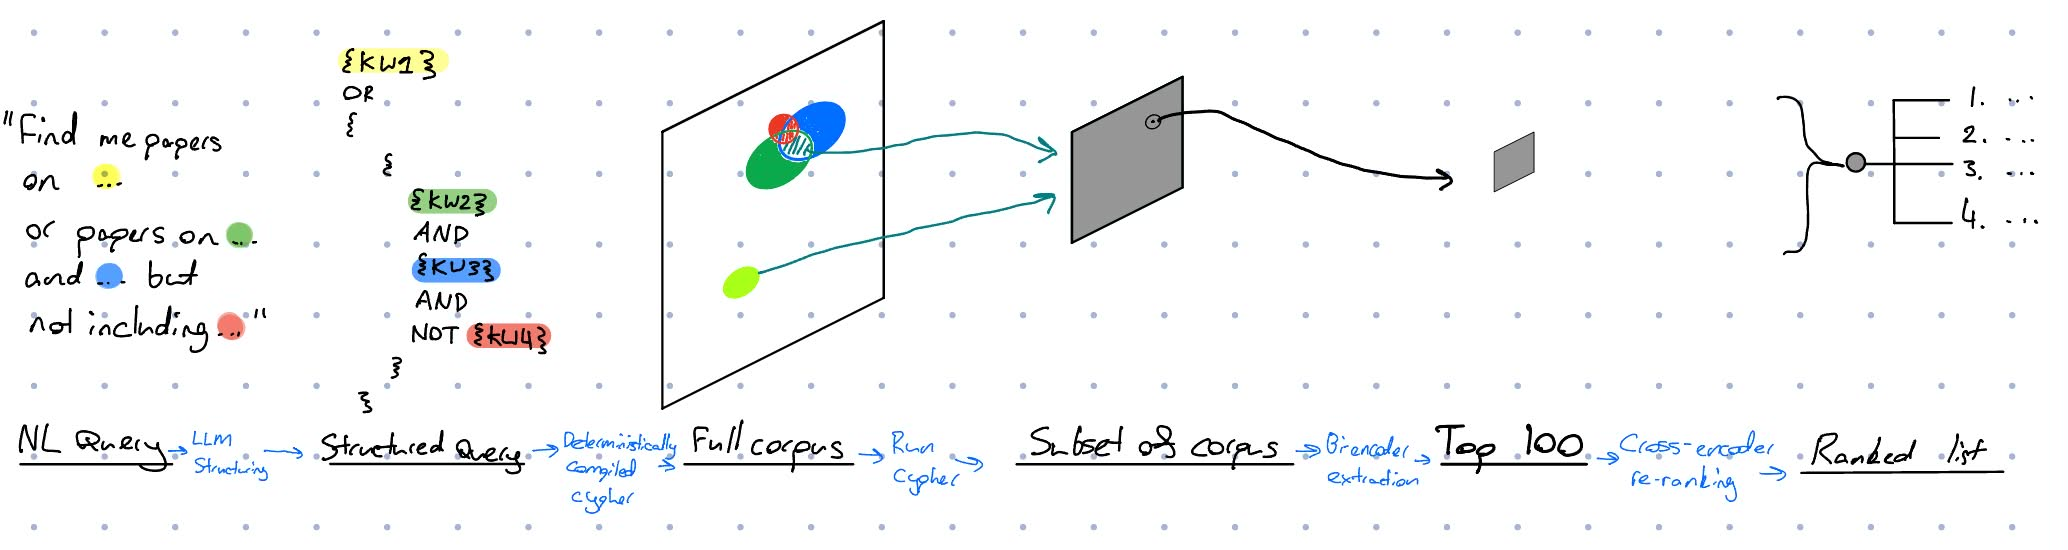
\includegraphics[width=\linewidth]{images/retrieval_pipeline.png}
    \caption{End-to-end representation of pipeline.}
    \label{fig:pipeline}
\end{figure}

\begin{table}[htbp]
    \centering
    \caption{Validation design}
    \label{tab:validation-design}
    \begin{tabularx}{\linewidth}{@{}p{2.4cm}%
        >{\raggedright\arraybackslash}X%
        >{\raggedright\arraybackslash}X%
        >{\raggedright\arraybackslash}X@{}}
        \toprule
        \textbf{Component} & \textbf{Validation Target} & \textbf{Dataset} & \textbf{Metric} \\
        \midrule
        Keyword extraction   & Keyword quality              & KPBiomed, OAGKX, PubMedAKE     & Present/absent F1@5 (stemmed)        \\
        IR extraction        & Query-understanding accuracy & Hand-built stratified gold set & Entity match + logical equivalence   \\
        Dense bi-encoder     & Retrieval quality            & SciRepEval ad-hoc search       & nDCG                                 \\
        Cross-encoder        & Re-ranking quality           & SciRepEval ad-hoc search       & nDCG                                 \\
        Embedding quantisation & Int8 accuracy cost         & SciRepEval ad-hoc search       & nDCG (fp32 vs.\ int8)                \\
        \bottomrule
    \end{tabularx}
\end{table}

Each component designed in Section~\ref{subsec:component-design} is validated independently, against established benchmarks to allow for a comparison of models, from which one can be selected for the final system. This component-wise validation strategy, as summarised in Table~\ref{tab:validation-design}, acts as the counterpart to the design outlined in Section~\ref{subsec:component-design}, following the design and validation approach of Section~\ref{subsec:design-approach}. The outcome of each benchmark, including the model selected, is reported in the Data and Results section.

\subsubsection{Keyword Generation}
\label{subsubsec:keyword-generation}

The keyword generation module of Section~\ref{subsubsec:ingestion-storage} is evaluated against three keyphrase datasets, namely KPBiomed, OAGKX, and PubMedAKE, each of which pairs documents with reference keyphrases. Reference keyphrases are split into present (extractive) keyphrases, which occur verbatim in the source text, and absent (abstractive) keyphrases, which do not and so must be generated. Each is scored by F1@5 with light stemming, so that a keyphrase and its stem count as a match while a different word of the same meaning does not. The present/absent split isolates faithful extraction from generation, which matters because a language-model extractor can hallucinate keyphrases the source does not contain. 

The candidates place a large-language-model generator, GPT-5.4-nano, against established statistical and neural baselines: TF-IDF, YAKE, TextRank, and MultipartiteRank as statistical or graph-based extractors; KeyBERT-MiniLM and KBIR-inspec as neural extractors; and KeyBART as a fine-tuned generative model. The purely extractive baselines can match only present keyphrases by construction, whereas the generative models can also attempt absent ones, so the present/absent split doubles as a comparison between the two families.

\subsubsection{IR Extraction}
\label{subsubsec:ir-extraction}

This benchmark measures how well the model turns an unstructured query into the structured nested boolean representation, the IR (Section~\ref{subsubsec:structured-retrieval}). The model's output is compared against a correct IR written by hand, an approach known as intrinsic evaluation, rather than judging the model by the quality of the final search results. This is done to separate the two possible sources of error. If the system were judged only on its final results, a poor result could come from a mistake in the translation step or in the later search stages, with no way to tell which. Comparing against a correct IR measures the translation step on its own.

The benchmark was built by hand, because the literature (Section~\ref{sec:lr-gap}) found that no existing benchmark covers this task in the scholarly domain. It was constructed as follows:

\begin{itemize}
    \item A set of sample queries was curated to match the vocabulary expected of users, including technical keywords, researcher names, institutions, and venues, so that every entity type the system supports is exercised. The queries span a range of difficulty, from a single topic, through queries that combine topics with AND, OR, and NOT, up to queries that group these with brackets. The simple queries were taken from an existing retrieval dataset, SciRepEval, and the harder ones, which everyday queries rarely contain, were based on the structure of expert queries written for systematic reviews, the exhaustive evidence searches common in fields like medicine.
    \item For each query, the correct nested boolean representation was written by hand. Where a query was ambiguous in how its terms should be grouped, the wording was tightened or brackets were added, so that each query has a single intended answer.
\end{itemize}

Each model is then scored against the hand-written answers on two parts. The first is the entities, the individual terms the model pulled out. These are compared to the correct terms allowing small surface differences, such as a word and its stem, but not accepting a different word of the same meaning, since this stage is meant to capture the terms the user actually wrote rather than paraphrase them. The second is the expression, the way those terms are combined with AND, OR, and NOT. This is judged by logical equivalence, meaning the answer counts as correct if it selects the same papers as the hand-written one, even when written in a different but equivalent form. The same request can be arranged in more than one valid way, for example A AND B is the same as B AND A. Several candidate models are scored this way, with the selected model and the scores reported in the Data and Results section.

\subsubsection{Dense Retrieval}
\label{subsubsec:dense-retrieval}

The dense bi-encoder is evaluated on the ad-hoc search tasks of SciRepEval, namely NFCorpus, TREC-CoVID, and Search, measured by nDCG. SciRepEval is an established benchmark for scientific document retrieval (Section~\ref{sec:lr-bench}), and nDCG is the standard measure of ranking quality, which keeps the stage comparable to prior work. 

The candidates comprise general-purpose embedders (Qwen3-Embedding at 0.6B and 4B, EmbeddingGemma-300M, mxbai-embed-large-v1, BGE-M3, and the hosted text-embedding-3-small) alongside the scientific fine-tuned SPECTER2 in both its base and ad-hoc-query variants. The set contrasts general-purpose against domain-tuned encoders, and self-hostable against paid-API models (text-embedding-3-small being the sole hosted option), the two axes along which the results divide.

\subsubsection{Cross-Encoder Re-ranking}
\label{subsubsec:cross-encoder}

The cross-encoder is evaluated on the same SciRepEval ad-hoc search tasks under the same metric, by re-ranking the retrieved candidates, so the gain it adds can be read directly against the bi-encoder alone. 

Thirteen rerankers are compared: commercial APIs (Cohere Rerank 4.0 in its Pro and Fast tiers); self-hostable neural rerankers (the Qwen3-Reranker at 0.6B and 4B, jina-reranker-v2, and mxbai-rerank-large-v1); a biomedical domain-specific model (MedCPT); and older cross-encoder baselines (the ms-marco-MiniLM and bge-reranker families, and gte-reranker-modernbert-base). This spread lets the results separate model family and recency from raw parameter count, and general-purpose rerankers from the domain-specific one.

\subsubsection{Embedding Quantisation}
\label{subsubsec:embedding-quantisation}

Quantising the embeddings to int8 (Section~\ref{subsubsec:ingestion-storage}) trades precision for memory, so its cost is measured rather than assumed. The bi-encoder evaluation above is repeated with the embeddings held at int8 and compared against the full-precision result, and the resulting difference in nDCG is the accuracy cost attributed to the quantisation.

\subsubsection{System-Level Evaluation}
\label{subsubsec:system-level}

The composed system has no off-the-shelf end-to-end benchmark, which reflects the gap identified in Section~\ref{sec:lr-limitations}. Under the separation of concerns above, however, the system's behaviour follows from its parts. The structured stage returns the papers matching the boolean query, established by the IR and keyword evaluations together with the deterministic compiler, and the dense stages rank those papers, established by their benchmarks. The component results therefore stand as the primary evidence for the system, subject to two limits stated plainly. First, the dense models are benchmarked on a full corpus rather than on the candidate set they rank within the cascade, so their measured quality is a close proxy for their role here rather than a direct measurement of it. Second, the system returns only papers that match the boolean query, so a paper that is relevant but does not match is not retrieved, which is the precision-oriented behaviour the design intends rather than a defect. A system-level evaluation confirms both points directly: the assembled cascade is compared against a retrieval-augmented LLM and Google Scholar over a curated set of realistic queries, assessed qualitatively per query and with light relevance judgments over the returned results. This comparison is the instrument for RQ3; its results appear in Section~\ref{sec:results-system} and its analysis in Section~\ref{subsec:rq3}.